% Concept addition as vector addition.
% An activation h is shifted by alpha*c along a concept direction c. Because c
% has a positive component along w_r, the projection onto w_r grows: the reward
% goes up by alpha * w_r^T c.
% Compile with ../build_figures.sh -> content/assets/figures/concept-vector.svg
\documentclass[border=10pt]{standalone}
\usepackage{tikz}
\usetikzlibrary{calc,arrows.meta}
\definecolor{rlink}{HTML}{3F51B5}    % reward direction
\definecolor{raccent}{HTML}{FF5722}  % the increase in reward
\definecolor{rmuted}{HTML}{6B7280}
\begin{document}
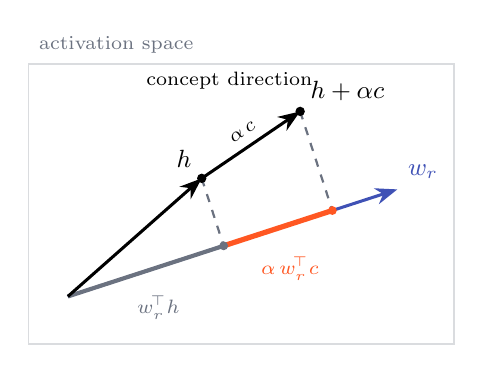
\begin{tikzpicture}[>=Stealth, line width=0.9pt, font=\small]
  \coordinate (O)  at (0,0);
  \coordinate (W)  at (18:4.4);
  \coordinate (H)  at (1.7,1.5);       % activation h
  \coordinate (HC) at (2.95,2.35);     % h + alpha c
  \coordinate (FH) at ($ (O)!(H)!(W) $);    % foot of h on the reward axis
  \coordinate (FC) at ($ (O)!(HC)!(W) $);   % foot of h + alpha c

  % activation-space frame
  \draw[rmuted!25, line width=0.6pt] (-0.5,-0.6) rectangle (4.9,2.95);
  \node[rmuted, font=\scriptsize, anchor=south west] at (-0.5,2.95) {activation space};

  % reward direction (thin, so the orange increase reads on the axis)
  \draw[rlink, ->, line width=1.1pt] (O) -- (W) node[above right, rlink] {$w_r$};

  % orthogonal drops onto the reward axis
  \draw[rmuted, dashed, line width=0.8pt] (H)  -- (FH);
  \draw[rmuted, dashed, line width=0.8pt] (HC) -- (FC);

  % baseline projection of h, then the orange increase from adding the concept
  \draw[rmuted, line width=1.5pt] (O) -- (FH);
  \draw[raccent, line width=1.9pt] (FH) -- (FC);

  % the activation and the concept step
  \draw[black, ->, line width=1.1pt] (O) -- (H);
  \draw[black, ->, line width=1.1pt] (H) -- (HC)
     node[midway, above, sloped, black, font=\scriptsize] {$\alpha\,c$};
  \node[black, font=\scriptsize, anchor=south] at (2.05,2.5) {concept direction};

  % points
  \fill (H)  circle (1.7pt) node[above left, black] {$h$};
  \fill (HC) circle (1.7pt) node[above right, black] {$h+\alpha c$};
  \fill[rmuted]  (FH) circle (1.6pt);
  \fill[raccent] (FC) circle (1.6pt);

  % labels for the two segments on the axis
  \node[rmuted, font=\scriptsize, anchor=north] at (1.15,0.14) {$w_r^{\!\top} h$};
  \node[raccent, font=\scriptsize, anchor=north] at (2.82,0.64) {$\alpha\,w_r^{\!\top} c$};
\end{tikzpicture}
\end{document}
